% !TEX root = ../notes_template.tex

\chapter{복소미분}

이 장에서는 다음 3가지 주제를 중점적으로 다룬다.




\begin{figure}[!h]
\begin{center}
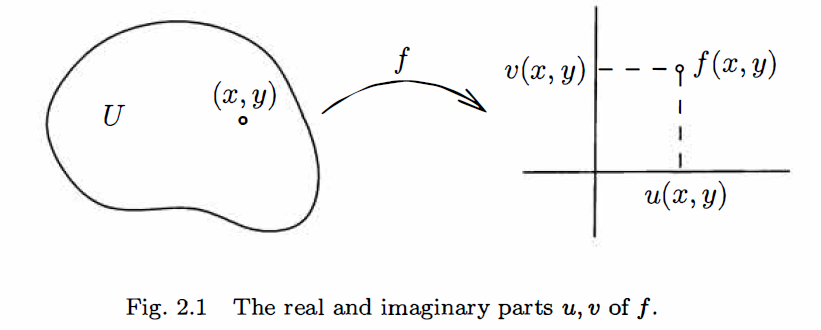
\includegraphics[width=0.6\textwidth]{./SaltChapter/fig-2-1}
\end{center}
\caption{$f$의 실수부와 허수부 $u$, $v$}
\label{fig-2-1}
\end{figure}



\begin{salt_exercise} \label{ex-1-4}
다음 복소수를 복소평면 위의 점으로 표시하라.
$$
0, \quad 1 , \quad -\frac32, \quad i, \quad -\sqrt{2}i,
\quad \cos \frac\pi3 + i\sin\frac\pi3.
$$
\end{salt_exercise}